% !TeX spellcheck = cs_CZ
%{\tikzset{external/prefix={tikz/FYZII/}}
% \tikzset{external/figure name/.add={ch03_}{}}
%---------------------------------------------------------------------------------------------------
% file fey1ch01_02_03.tex
%---------------------------------------------------------------------------------------------------
%================= Kapitola: Integrální počet vektorových polí =====================================
\setchaptertoc
\chapter{Integrální počet vektorových polí}\label{fyz:IIchapIII}


  %------------ Vektorový integrály, křivkový integrál \(\nabla\Psi\) ------------------------------
  \section{Vektorové integrály, křivkový integrál \texorpdfstring{\(\nabla\Psi\)}{nabla 
  psi}}\label{fyz:IIchapIIIsecI}
    V kapitole \ref{fyz:IIchapII} jsme viděli, že existují různé způsoby derivování polí. Některé 
    vedou k vektorovým polím, jiné dávají pole skalární. Ačkoliv jsme odvodili mnoho různých 
    vzorců, vše, co je v kapitole \ref{fyz:IIchapII}, lze shrnout do jediného pravidla: operátory 
    \(\pder{ }{x}\), \(\pder{ }{y}\) a \(\pder{ }{z}\) představují tři složky vektorového operátoru 
    \(\nabla\). Rádi bychom nyní trochu vnikli do významu derivací polí. Potom získáme lepší cit 
    pro to, co znamená vektorová rovnice pole.
    
    Již jsme se zmínili o významu operace gradient (\(\nabla\) působí na skalár). Teď se budeme  
    zajímat o význam operací divergence a rotace. Interpretovat tyto veličiny je možné nejlépe 
    pomocí určitých vektorových integrálů a rovnic, které uvádějí tyto integrály do souvislosti. 
    Bohužel, tyto rovnice nelze získat z vektorové algebry nějakou snadnou substitucí. Proto si je 
    odvodíme a objasníme, co z nich vyplývá. Rovnice, které budeme studovat, představují vlastně 
    matematické věty. Užitečné budou nejen při interpretování významu a obsahu divergence a rotace, 
    ale i při vypracování obecných fyzikálních teorií. Tyto matematické věty jsou pro teorii polí 
    tím, čím je zákon zachování energie pro mechaniku částic. Takové obecné věty, jako jsou tyto, 
    jsou důležité pro hlubší porozumění fyziky. Uvidíme však, že při řešení úloh z nich mnoho 
    užitku není (s výjimkou nejjednodušších případů). I tak je potěšující, že na začátku našeho 
    výkladu se setkáme s mnoha jednoduchými úlohami, řešitelnými pomocí těchto tří integrálních 
    vzorců, které budeme nyní probírat. Uvidíme však, že sotva se úlohy stanou těžšími, nebudeme 
    moci tyto jednoduché metody použít.

    Nejdříve si vezměme integrální vzorec s gradientem. Obsahuje velmi jednoduchou myšlenku: 
    Protože gradient představuje rychlost změny veličiny mající charakter pole, inte\-gru\-jeme-li 
    tuto rychlost změny, dostaneme celkovou změnu. Předpokládejme, že máme skalární pole \(\Psi(x, 
    y, z)\). Funkce \(\Psi\) bude mít v nějakých dvou bodech \((1)\) a \((2)\) hodnoty \(\Psi(1)\), 
    resp. \(\Psi(2)\) (Používáme symboliku, ve které \((2)\) představuje bod \(x_2, y_2, z_2\) a 
    \(\Psi(2)\) znamená totéž jako \(\Psi(x_2, y_2, z_2)\).) Je-li \(\Gamma\)(gama) nějaká 
    křivka spojující body \((1)\) a \((2)\) (obr. \ref{fyz:fig033}), platí následující
    \begin{equation}\label{fyz:eq275}
      \Psi(2)-\Psi(1) = \int_{\substack{(1)\\\text{po }\Gamma}}^{(2)}(\nabla\Psi)\cdot\dd{\vec{s}}
    \end{equation} 

    \begin{figure}[ht!] 
      \centering
      \subcaptionbox{\label{fyz:fig033}}{\luafigure[0.45]{fyz_fig033_1.pdf}}
      \subcaptionbox{\label{fyz:fig157}}{\luafigure[0.45]{fyz_fig157_1.pdf}}
      \caption{a) Význam veličin vystupujících v rovnosti \ref{fyz:eq275}. Vektor 
      \(\nabla\Psi\) se vztahuje k elementu \(ds\). b) Křivkový integrál je limitou součtu. 	
               (\cite[s.~46]{Feynman02})}
    \end{figure}

    Jde o \emph{křivkový integrál} z \((1)\) do \((2)\) skalárního součinu \(\nabla\Psi\) (vektor) a
    \(d\vec{s}\) (jiný vektor - infinitezimální element křivky \(\Gamma\), orientovaný ve směru  
    postupu z \((1)\) do \((2)\) po křivce \(\Gamma\)).
    
    Nejdříve bychom měli vysvětlit, co rozumíme křivkovým integrálem. Uvažujme skalární funkci 
    (\(x\), \(y\), \(z\)) a křivkxu \(\Gamma\) spojující dva body \((1)\) a \((2)\). Vyznačme na 
    křivce nějaký počet bodů a sousední body spojujeme tak, jak ukazuje obr.  \ref{fyz:fig157}. 
    Délku jednotlivých úseček označme \(\Delta s_i\) kde \(i\) je index, který nabývá hodnot 
    \(1,2,3,\ldots\). Křivkovým integrálem \(\displaystyle\int_{\substack{(1)\\\text{po 
    }\Gamma}}^{(2)}f\dd{s}\) rozumíme limitu součtu \(\displaystyle\sum_i f_i\Delta s_i\), kde 
    \(f_i\) je hodnota funkce pro \(i\)-tou úsečku. Limitní hodnota je to, čemu se součet blíží, 
    přidáváme-li víc a víc úseček (takovým způsobem, aby největší \(\Delta s_i\rightarrow 0\)).
    
    Integrál v naší větě (vztah \ref{fyz:eq275}) znamená totéž, ačkoli vypadá trochu jinak. Namísto 
    \(f\) máme jiný skalár - složku \(\Delta\Psi\) ve směru \(\Delta\vec{s}\). Označíme-li tuto 
    tangenciální složku \((\Delta\Psi)_t\), je jasné, že
    \begin{equation}\label{fyz:eq274}
      (\nabla\Psi)_t\Delta s = (\nabla\Psi)\cdot\Delta\vec{s}
    \end{equation}
    Integrál v (\ref{fyz:eq274}) představuje sumu takovýchto členů.
    
    Nyní se podívejme na to, proč rovnost (\ref{fyz:eq274}) platí. V kapitole   
    \ref{fyz:IIchapI} je ukázáno, že složka \(\Delta\Psi\) ve směru malého posunutí 
    \(\Delta\vec{r}\) udává rychlost změny \(\Psi\) v tomto směru \(\Delta\vec{r}\). Uvažujme o 
    úsečce \(\Delta\vec{s}\) z bodu \((1)\) do bodu \(a\) na obr. \ref{fyz:fig157}. Podle 
    naší definice  
    \begin{align}
     \Delta\Psi_1 = \Psi(a) - \Psi(1) 
       &= (\nabla\Psi)_1\cdot\Delta\vec{s_1}.         \label{fyz:eq267a}  \\
     \shortintertext{Taktéž}
     \Psi(b) - \Psi(a)
       &= (\nabla\Psi)_2\cdot\Delta\vec{s_2},         \label{fyz:eq267b}
    \end{align}
    kde \((\nabla\Psi)_1\), znamená, samozřejmě, gradient počítaný na úsečce \(\Delta\vec{s_1}\) a 
    \((\nabla\Psi)_2\) gradient počítaný na úsečce \(\Delta\vec{s_2}\). Výpočtem rovností 
    (\ref{fyz:eq267a}) a (\ref{fyz:eq267b}) dostaneme
    \begin{align}
     \Psi(b) - \Psi(1)              &= 
        (\nabla\Psi)_1\cdot\Delta\vec{s_1} + 
        (\nabla\Psi)_2\cdot\Delta\vec{s_2}               \label{fyz:eq268a} \\
     \shortintertext{Můžeme se přesvědčit, že postupným přidáváním takovýchto členů dostaneme}
     \Psi(2) - \Psi(1)              &= 
       \sum_i(\nabla\Psi)_i\cdot\Delta\vec{s_i}          \label{fyz:eq268b}
    \end{align}
    Levá strana nezávisí na tom, jak volíme naše intervaly (zů\-stá\-va\-jí-li body \((1)\) a 
    \((2)\) stejné) takže můžeme vzít limitu druhé strany. Tím jsme dokázali rovnost 
    (\ref{fyz:eq275}). Z našeho důkazu můžete vidět, že tato rovnost nezávisí ani na 
    tom, jak zvolíme body \(a\), \(b\), \(c\) ..., ani na volbě křivky \(\Gamma\) spojující \((1)\) 
    a \((2)\). Naše věta platí pro jakoukoliv křivku vedenou z \((1)\) do \((2)\).
    
    Ještě jedna poznámka o označování: Uvidíme, že nevznikne žádný zmatek, budeme-li pro pohodlí psát
    \begin{equation}\label{fyz:eq269}
     (\nabla\Psi)\cdot\dd{\vec{s}} = \nabla\Psi\cdot\dd{\vec{s}}
    \end{equation}     
    V tomto označení má naše věta tento tvar:
    \begin{equation}\label{fyz:eq273}
     \Psi(2)-\Psi(1) =  
       \limitint_{\mathclap{\substack{(1)\\\text{jakákoli křivka}\\\text{od (1) do 
       (2)}}}}^{(2)}
         \nabla\Psi\cdot\dd{\vec{s}}
    \end{equation}

  %---------------------- Tok vektorového pole -----------------------------------------------------
  \section{Tok vektorového pole}\label{fyz:IIchapIIIsecII}
    Definovali jsme vektor $\vec{h}$ jako teplo procházející jednotkovou plochou za jednotkový čas.
    Předpokládejme, že uvnitř tělesa vyplněného látkou máme nějakou uzavřenou plochu \(S\), která 
    ohraničuje objem \(V\). Chtěli bychom zjistit, kolik tepla vytéká z tohoto objemu.
    
    Označme plošný obsah elementu plochy \(S\) jako \(dS\). Tento symbol nahrazuje dvojrozměrný
    diferenciál
    \begin{equation}
      ds=dx\,dy.
    \end{equation}
    Tok tepla elementární ploškou \(dS\) je roven jejímu plošnému obsahu  vynásobenému složkou 
    $\vec{h}$ kolmou na \(dS\). Už jsme definovali $\vec{n}$ jako jednotkový vektor směřující pod 
    pravým úhlem ven z plochy (obr. \ref{fyz:fig034}). Složka $\vec{h}$, kterou potřebujeme, je
    \begin{equation}
      h_n = \vec{h}\cdot\vec{n}
    \end{equation}
    Tok ploškou $dS$ pak je
    \begin{equation}\label{fyz:eq_int_fey_dS}
      \vec{h}\cdot\vec{n}\cdot\dd{S}
    \end{equation}
    Celkový tepelný tok jakoukoliv plochou dostaneme, sečteme-li příspěvky všech elementárních 
    plošek vytvářející plochu \(S\). Jinými slovy, integrujeme-li \ref{fyz:eq_int_fey_dS} přes 
    celou plochu: Celkový tepelný tok plochou \(S\) se rovná
    \begin{equation}
      \oint_S\vec{h}\cdot\vec{n}\dd{S}
    \end{equation}

    Tento plošný integrál\footnote{Malý kroužek na znaku integrálu znamená, že integrujeme přes 
    uzavřenou plochu.} budeme také nazývat \emph{tokem plochou}. Můžeme to chápat tak, že $\vec{h}$ 
    je hustota proudu tepelného toku a plošný integrál z ní je celkový proud tepla směřující ven z 
    plochy za jednotku času (v joulech za sekundu).
    
    Rádi bychom tuto ideu zobecnili na případ, kdy vektor nepředstavuje tok něčeho konkrétního, 
    mohlo by jít například o elektrické pole. Kdybychom chtěli, jistě bychom mohli integrovat 
    normálovou složku elektrického pole plochou. Ačkoliv tu nejde o tok něčeho, nazýváme tuto 
    veličinu tokem. Říkáme tok vektoru $\vec{E}$ plochou \(S\) se rovná 
    \(\int_S\vec{E}\cdot\vec{n}\dd{S}\). Slovo tok zde používáme v obecném významu jako, 
    \emph{plošný integrál normálové složky vektoru}.  
    
    \begin{figure}[ht!]
      \centering
      \subcaptionbox{\label{fyz:fig034}}{\luafigure[0.7]{fyz_fig034.pdf}}    \newline 
      \subcaptionbox{\label{fyz:fig214}}{\luafigure[0.7]{fyz_fig214.pdf}}
      \caption{a) Uzavřená plocha $S$ vymezuje objem $V$. Jednotkový vektor $\protect\vec{n}$ udává
              vnější normálu k plošnému elementu $dS$ a $\protect\vec{h}$ je vektor hustoty
              tepelného toku pro uvažovaný plošný element. b) Objem $V$ uvnitř plochy $S$ je řezem
              $S_{ab}$ rozdělen na dvě části. Dostáváme tím objem $V_1$ vymezený plochou
              $S_1=S_a+S_{ab}$ a objem $V_2$ vymezený plochou $S_2=S_b+S_{ab}$.
              \cite[s.~48]{Feynman02}}
    \end{figure}
    
    Vraťme se k případu tepelného toku a uvažujme situaci, v níž se teplo zachovává. Například si
    představíme nějakou látku, ve které se po počátečním ohřevu tepelná energie dále ani 
    negeneruje, ani neabsorbuje. Existuje-li pak tok tepla uzavřenou plochou, musí tepelný obsah 
    objemu vymezeného plochou klesat. Tedy v podmínkách, ve kterých se teplo zachovává, tvrdíme, že
    \begin{equation}\label{fyz:eq_int_fey_dQ}
      \oint_S\vec{h}\cdot\vec{n}\cdot\dd{S} = - \frac{dQ}{dt}
    \end{equation}
    kde $Q$ je teplo uvnitř plochy. Tok tepla plochou $S$ je roven rychlosti změny celkového tepla 
    $Q$ uvnitř $S$ za čas, vzaté se záporným znaménkem. Takováto interpretace je možná, neboť 
    hovoříme o tepelném toku a kromě toho jsme udělali předpoklad, že teplo se zachovává. O 
    celkovém teple uvnitř objemu bychom nemohli hovořit, kdyby se v tomto objemu teplo generovalo.
    
    Nyní poukážeme na zajímavou vlastnost toku jakéhokoliv vektoru. Můžeme mít na mysli stále 
    vektor tepelného toku, ale vše bude platit i pro jakékoliv vektorové pole $\vec{C}$. Představme 
    si, že máme uzavřenou plochu $S$, která ohraničuje objem $V$. Rozdělme nyní objem $V$ jakýmsi 
    řezem na dvě části (obr. \ref{fyz:fig214}). Dostaneme tím dvě uzavřené plochy a dva objemy. 
    Objem $V_1$ ohraničuje plocha $S_1$, která se skládá ze zbytku původní plochy $S_a$ a plochy 
    řezu $S_{ab}$. Objem $V_2$ ohraničuje plocha $S_2$, která se skládá ze zbytku původní plochy 
    $S_b$ doplněné řezem $S_{ab}$. Položme si nyní otázku: Předpokládejme, že vypočítáme tok z 
    plochy $S_1$ a přičteme ho k toku z plochy $S_2$. Je roven tento součet toku z celé plochy $S$, 
    s níž jsme původně začínaly? Odpověď zní ano. Tok z částí ploch $S_{ab}$, společnou oběma 
    plochám $S_1$ a $S_2$ se přesně vyruší. Pro tok vektoru $\vec{C}$ z objemu $V_1$ můžeme psát:
      
    \begin{itemize}
      \item tok plochou $S_1$ je roven:
        \begin{equation}\label{fyz:eq_int_Sa}
           \int_{S_a}\vec{C}\cdot\vec{n}\dd{S} + \int_{S_{ab}}\vec{C}\cdot\vec{n_1}\dd{S}
        \end{equation}
      \item tok plochou $S_2$ je roven:
         \begin{equation}\label{fyz:eq_int_Sb}
           \int_{S_b}\vec{C}\cdot\vec{n}\dd{S} + \int_{S_{ab}}\vec{C}\cdot\vec{n_2}\dd{S}
        \end{equation}
    \end{itemize} 
    Všimněme si, že v druhém integrálu jsme psali $\vec{n_1}$, pro vnější normálu k $S_{ab}$, 
    patří-li tato k $S_1$ a $\vec{n_2}$ patří-li k $S_2$, jak ukazuje obr. \ref{fyz:fig214}. 
    Zřejmě $\vec{n_1}= -\vec{n_2}$ takže
    \begin{equation}
    \int_{S_{ab}}\vec{C}\cdot\vec{n_1}\dd{S} = - \int_{S_{ab}}\vec{C}\cdot\vec{n_2}\dd{S}
    \end{equation}
    Sečteme-li rovnosti \ref{fyz:eq_int_Sa} a \ref{fyz:eq_int_Sb} přesvědčíme se, že součet toku 
    přes $S_1$ a $S_2$ je dán součtem dvou integrálů, které spolu dávají tok původní plochy $S = 
    S_a + S_b$.
    
    Vidíme, že o toku úplnou vnější plochou $S$ je možné uvažovat jako o součtu toků dvou částí, na 
    které se objem $V$ rozdělil. \emph{Takto pro jakýkoliv způsob dělení původního objemu musí 
    obecně platí, že tok vnější plochou, daný původním integrálem, je roven součtu toků ze všech 
    jeho malých vnitřních částí.} 
    
  %------------------- Tok povrchem krychle. Gaussova věta------------------------------------------
  \section{Tok povrchem krychle. Gaussova věta}\hypertarget{fyz:IIchapIIIsecIII}
    Uvažujme krychli jejíž hrany mají směr souřadnicových os tak, jako na obr. 
    \ref{fyz:fig215}. Předpokládejme, že souřadnice jednoho z vrcholu krychle je totožný 
    se začátkem souřadnicové soustavy $x,y,z$. Nechť $\Delta x$ je délka hrany krychle ve směru osy 
    $x$, $\Delta y$ je délka hrany ve směru osy $y$ a $\Delta z$ délka hrany ve směru osy $z$. 
    Chceme najít tok vektorového pole \(\vec{C}\) povrchem krychle. Dostaneme jej sečtením toků 
    každou ze šesti stěn. Nejdříve uvažujeme stěnu na obrázku \ref{fyz:fig215} označenou 
    jako $1$. Tok směřující touto stěnou ven z krychle je dán integrálem záporně vzaté x-ové složky 
    \(\vec{C}\) plochou stěny: Protože máme malou krychli můžeme tento integrál aproximovat 
    hodnotou $x$ ve středu stěny (označíme jej jako bod $1$) vynásobenou plošným obsahem stěny, tj. 
    $\Delta y 
    \Delta z$:        
    \begin{align}
      \text{tok z 1} &= -C_x\Delta y \Delta z                                           \\
      \intertext{Podobně napíšeme tok stěnou $2$:}
      \text{tok z 2} &= C_x\Delta y \Delta z                                            \\
      \intertext{Obecně se $C_x(1)$ a $C_x(2)$ trochu liší. Je-li dostatečně malé, můžeme psát}
       C_x(2)        &= C_x(1) + \pder{C_x}{x}\Delta x.                             
    \end{align}            
    \noindent Na pravé straně tohoto vztahu bychom ve skutečnosti měli uvést víc členů. Všechny 
    však budou obsahovat vyšší mocniny $\Delta x$, a proto, uvažujeme-li limitní případ malého 
    $\Delta x$, budou zanedbatelné. Takovým způsobem pro tok stěnou $2$ vychází
    \begin{align}    
      \text{tok z 2} &= \left(C_x(1) + \pder{C_x}{x}\Delta x\right)\Delta y \Delta z.             \\
      \intertext{Sečtením toků stěnami $1$ a $2$ dostaneme}
      \text{tok z 1 a 2} &= \pder{C_x}{x}\Delta x\Delta y\Delta z.
    \end{align}      
    
    \luagraphic[1]{fyz_fig215.pdf}{Výpočet toku pole \(\vec{C}\) z malé krychle}{fyz:fig215}
    
    Derivace by se měla počítat ve skutečnosti ve středu stěny $1$, tj v bodu $[x, y+\frac{\Delta 
    y}{2}, z + \frac{\Delta z}{2}]$. Ale v limitním případě infinitezimální krychle uděláme pouze 
    zanedbatelnou chybu, počítáme-li je ve vrcholu $(x,y,z)$.
    
    Provedeme-li stejné úvahy pro každý z dvou párů stěn, dostaneme    
    \begin{align*}
     \text{tok z 3 a 4} &= \pder{C_y}{y}\Delta x\Delta y\Delta z   \\ 
     \text{tok z 5 a 6} &= \pder{C_z}{z}\Delta x\Delta y\Delta z.
    \end{align*}       
    Celkový tok všemi stěnami je součtem těchto členů. Dostáváme tedy
    \begin{equation}
     % source http://texblog.net/latex-archive/graphics/tikz-cube-3d/
     \limitint_{\mathclap{\substack{\text{\ding{114}}}}}\vec{C}\cdot\vec{n}\dd{S}
        = \left(\pder{C_x}{x}+\pder{C_y}{y} +
          \pder{C_z}{z}\right)\Delta x\Delta y \Delta z.
    \end{equation}
    Součtem derivací je právě $\nabla\cdot\vec{C}$ a dále $\Delta x\Delta y \Delta z = \Delta V$, 
    tj objem krychle. Takovýmto způsobem můžeme pro infinitezimální krychli psát
    \begin{equation}
      \limitint_{\mathclap{\substack{\text{\ding{114}}}}}\vec{C}\cdot\vec{n}\dd{S}
       = (\nabla\cdot\vec{C})\Delta V.       \label{fyz:eq_gauss1}
    \end{equation}
    
    Ukázali jsme, že tok z povrchu infinitezimální krychle ven je roven divergenci vektoru násobené 
    objemem krychle. Nyní vidíme význam divergence vektoru. Divergence vektoru v bodě \(P\) je tok 
    - vycházející „proud“ vektoru $\vec{C}$ - připadající na jednotkový objem v okolí \(P\).
    
    Divergenci \(\vec{C}\) jsme uvedli do souvislosti s tokem \(\vec{C}\) z každého 
    infinitezimálního objemu. V případě konečného objemu můžeme využít fakt, který jsme už 
    dokázali, že celkový tok z objemu je součtem toků z každé jedné části. To znamená, že 
    divergenci můžeme integrovat přes celý objem. Z toho vyplývá věta, že integrál normálové složky 
    každého vektoru přes jakoukoliv uzavřenou plochu je možné zapsat jako integrál z divergence 
    tohoto vektoru přes objem uzavřený touto plochou. Tato věta byla pojmenována po Gaussovi.
    \begin{equation}\label{fyz:eq_gauss_veta}
     \oint_S \vec{C}\cdot\vec{n}\dd{S} 
       = \int_V (\nabla\cdot\vec{C})\dd{V}, \quad\ldots\text{Gaussova věta}
    \end{equation}
    kde $S$ je jakákoliv uzavřená plocha a $V$ je objem jí vymezený.
    
    %--------------- Tepelná vodivost, rovnice difúze věta------------------------------------------
    \subsection{Tepelná vodivost, rovnice difúze}
      Abychom se lépe seznámili s \emph{Gaussovo větou}, uveďme nějaký případ jejího použití. 
      Vezměme opět případ tepelného toku, například v kovu. Předpokládejme, že máme jednoduchou 
      situaci, kdy všechno teplo bylo přivedeno už dříve a těleso se nyní pouze ochlazuje. Žádné 
      zdroje tepla už nejsou, takže teplo se zachovává. Kolik je potom tepla uvnitř určitého 
      zvoleného objemu v libovolném čase? Množství tepla se musí zmenšovat, a to právě o množství, 
      které vytéká z objemu jeho povrchem. Kdyby byl náš objem malou krychlí, pak podle vztahu
      \ref{fyz:eq_gauss1} bychom napsali
      \begin{equation}\label{fyz:eq_gauss2}
       \text{tok 
       tepla}=\limitint_{\mathclap{\substack{\text{\ding{114}}}}}\vec{h}\cdot\vec{n}\dd{S} = 
       \int(\nabla\cdot\vec{h})\Delta V.
      \end{equation}
      Tato hodnota však musí být rovna rychlosti, kterou se teplo ztrácí z vnitřku krychle. Je-li 
      $q$ teplo připadající na jednotkový objem, $q\Delta V$ je teplo v krychli a rychlost jeho
      \emph{úbytku} je
      \begin{equation}\label{fyz:eq_gauss3}
       - \der{ }{t}(q\Delta V) = - \der{q}{t}\Delta V.
      \end{equation}
      Z porovnání rov. \ref{fyz:eq_gauss2} a \ref{fyz:eq_gauss3} vidíme, že 
      \begin{equation}\label{fyz:eq_gauss4}
        \nabla\cdot\vec{h} = - \frac{dq}{dt}. 
      \end{equation}
      Podotkněme, že rovnice tohoto tvaru se ve fyzice vyskytuje velmi často. Vyjadřuje \emph{Zákon 
      zachování}, v tomto případě \emph{Zákon zachování tepla}. Ve vztahu \ref{fyz:eq_int_fey_dQ} 
      jsme tentýž fyzikální jev vyjádřili jiným způsobem. Zde máme \emph{diferenciální} tvar zákona 
      zachování zatímco rovnost \ref{fyz:eq_int_fey_dQ} představuje jeho \emph{integrální} tvar.
      
      Rovnici (\ref{fyz:eq_gauss4}) jsme odvodili použitím vztahu (\ref{fyz:eq_int_fey_dQ}) na 
      infinitezimální krychli. Můžeme postupovat i obráceně. Pro velký objem \(V\) ohraničený 
      plochou \(S\) vyplývá z Gaussovy věty
      \begin{equation}\label{fyz:eq_gauss5}
        \oint_S\vec{h}\cdot\vec{n}\dd{S} = \int\nabla\cdot\vec{h}\dd{V}.
      \end{equation}
      
      Dosadíme-li sem z (\ref{fyz:eq_gauss4}), zjistíme, že integrál na pravé straně je právě
      \(-\dfrac{dQ}{dt}\) a opět dostaneme vztah (\ref{fyz:eq_int_fey_dQ}).
      
      Nyní uvažujme jiný případ. Představme si, že máme těleso vyplněné látkou s malou dutinou 
      uvnitř. Nechť v ní dochází k nějaké chemické reakci generující teplo. Nebo bychom si to mohli 
      představit tak, že tam jsou nějaké vodiče vedoucí k miniaturnímu odporu, který je zahříván 
      elektrickým proudem. Budeme předpokládat, že teplo se generuje prakticky v jednom bodě. Nechť 
      \(P\) označuje energii uvolněnou v tomto bodě za jednu sekundu. Dále budeme předpokládat, že 
      ve zbytku objemu se teplo zachovává a že generování tepla probíhalo velmi dlouho, takže se 
      teplota už nikde nemění. Otázka zní: Jak vypadá tepelný vektor \(\vec{h}\) na různých místech 
      kovu? Jaká je hustota tepelného toku v každém bodě?
      
      Víme, že integrujeme-li normálovou složku vektoru \(\vec{h}\) po uzavřené ploše, která 
      obklopuje zdroj, vždy dostaneme \(P\). Všechno teplo, které se generuje v bodovém zdroji, 
      musí vyjít povrchem, neboť jsme předpokládali, že tok je stálý. Máme těžkou úlohu najít 
      vektorové pole, které integrováno přes jakoukoliv plochu, dá vždy \(P\). Toto pole však 
      můžeme najít docela snadno, vezmeme-li v úvahu speciální plochu. Vezmeme kulovou plochu s 
      poloměrem \(R\) a se středem ve zdroji a budeme předpokládat, že proudění tepla je radiální 
      (obr. \ref{fyz:fig035}). Intuice nám napovídá, že vektor \(\vec{h}\) by měl 
      směřovat radiálně, jde-li o velké těleso a nejsme-li blízko stěn, a že ve všech bodech kulové 
      plochy by měl mít stejnou velikost. Vidíme, že na to, abychom našli odpověď, přidáváme k naší 
      matematice jisté množství dohadů - obyčejně nazývané „fyzikální intuice“.

      \begin{figure}[ht!]  %\ref{fyz:fig035}
        \centering
        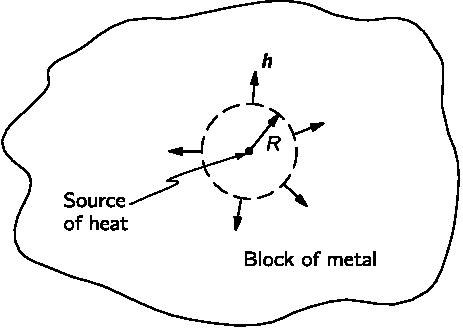
\includegraphics[width=0.6\linewidth]{fyz_fig035.pdf}
        \caption{V oblasti blízko bodového zdroje proudí teplo radiálně směrem ven.}
        \label{fyz:fig035}
      \end{figure}      
      Když je pole \(\vec{h}\) radiální a kulově symetrické, je integrál normálové složky vektoru 
      \(\vec{h}\) kulovou plochou velmi jednoduchý, protože tehdy je normálová složka vektoru rovna 
      velikosti vektoru \(\vec{h}\) a je konstantní. Obsah plochy, přes kterou integrujeme, je 
      \(4\pi R^2\). Potom dostaneme 
      \begin{equation}\label{fyz:eq_gauss6}
       \oint_S\vec{h}\cdot\vec{n}\dd{S} = h\cdot4\pi R^2
      \end{equation}
      kde \(h\) je velikost vektoru \(\vec{h}\). Tento integrál má být roven \(P\), tedy rychlosti, 
      se kterou teplo ve zdroji vzniká. Dostáváme
      \begin{align}
       h       &= \frac{P}{4\pi R^2}                \nonumber                  \\
       \shortintertext{nebo}
       \vec{h} &= \frac{P}{4\pi R^2}\vec{e_r}       \label{fyz:eq_gauss7}
      \end{align} 
      kde, jako obvykle, \(\vec{e_r}\) představuje jednotkový vektor v radiálním směru. Podle 
      našeho výsledku je \(\vec{h}\) přímo úměrné \(P\) a mění se nepřímo úměrně s druhou mocninou 
      vzdálenosti od zdroje.
      
      Výsledek, který jsme právě dostali, se hodí na proudění tepla v blízkosti bodového zdroje 
      tepla. Pokusme se nyní najít rovnice pro nejobecnější případ proudění tepla, platí-li jediná 
      podmínka, že teplo se zachovává. Budeme se zabývat pouze tím, co se stane v prostoru bez 
      jakýchkoliv zdrojů nebo absorbátorů tepla.
      
      Diferenciální rovnice pro vedení tepla byla odvozena v kapitole 
      \ref{fyz:IIchapII}. Podle rovnice (\ref{fyz:eq685}) platí
      \begin{equation}\label{fyz:eq_gauss8}
      \vec{h}=-\lambda\nabla T
      \end{equation}    
      (vzpomeňte si, že tento vztah platí sice přibližně, ale pro takové látky jako jsou kovy, 
      docela dobře.) Dá se použít, samozřejmě, jen v těch oblastech látky, ve kterých nedochází ke 
      generování nebo absorpci tepla. Už jsme odvodili jiný vztah, rovnici (\ref{fyz:eq_gauss4}), 
      který platí, když se teplo zachovává. Když v (\ref{fyz:eq_gauss4}) vektor \(\vec{h}\) 
      vyjádříme podle (\ref{fyz:eq_gauss8}), dostaneme
      \begin{align}
        - \der{q}{t} &= \nabla\cdot\vec{h} = - \nabla\cdot(\lambda\nabla T)     \nonumber    \\ 
        \intertext{nebo}
          \der{q}{t} &= \lambda\nabla\cdot\nabla T = \lambda\nabla^2 T     \label{fyz:eq_gauss9}
      \end{align}
      je-li \(\lambda\) konstanta. Vzpomínáte si, že \(q\) je množství tepla v jednotkovém objemu a
      \(\nabla\cdot\nabla = \nabla^2\) je \emph{Laplaceův operátor}
      \begin{equation*}
        \nabla^2= \pder{ }{x^2} + \pder{ }{y^2} + \pder{ }{z^2}.
      \end{equation*}       
    
      Uděláme-li ještě jeden předpoklad, můžeme dostat velmi zajímavou rovnici. Budeme 
      předpokládat, že teplota látky je přímo úměrná tepelnému obsahu jednotkového objemu, tj. že 
      látka má určitou  měrnou tepelnou kapacitu. Platí-li tento předpoklad (což bývá často), 
      můžeme psát
      \begin{align}
        \Delta q   &= c_V\Delta T                                        \nonumber    \\ 
        \intertext{nebo}
        \der{q}{t} &= c_V\der{T}{t}.                                     \label{fyz:eq_gauss10}
      \end{align}    
      Rychlost změny tepla je přímo úměrná rychlosti změny teploty. Součinitel úměrnosti \(c_V\) je 
      \emph{měrná tepelná kapacita jednotky objemu látky}. Ze vztahů (\ref{fyz:eq_gauss10}) a 
      (\ref{fyz:eq_gauss9}) 
      dostáváme
      \begin{equation}\label{fyz:eq_gauss11}
       \der{T}{t} = \frac{\lambda}{c_V}\nabla^2T
      \end{equation}
      Zjišťujme, že časová rychlost změny \(T\) v každém bodě je přímo úměrná Laplaceovu operátoru 
      teploty \(T\), tj. druhé derivaci její závislosti na poloze v prostoru. Dostáváme 
      diferenciální rovnici s proměnnými \(x\), \(y\), \(z\) a \(t\) pro teplotu \(T\).
      
      Diferenciální rovnice (\ref{fyz:eq_gauss11}) se nazývá \emph{rovnicí difúze tepla}. Často je 
      psána ve tvaru
      \begin{equation}\label{fyz:eq_gauss12}
       \der{T}{t} = D\nabla^2T
      \end{equation}
      kde \(D\) je koeficient \emph{difúze} tepla a zde je roven hodnotě
      \(\displaystyle\frac{\lambda}{c_V}\).
      
      Rovnice difúze se objevuje v mnoha fyzikálních úlohách - při difúzi plynů, neutronů a v 
      dalších případech. Nyní však máme úplnou rovnici, která popisuje difúzi v nejobecnější možné 
      situaci. Později probereme způsoby řešení rovnice difúze, abychom našli, jak se v konkrétních 
      případech mění teplota. Nyní se vrátíme zpět k výkladu dalších vět o vektorových polích.

  %------------- Cirkulace vektorového pole ------------------------------------------------------- 
  \section{Cirkulace vektorového pole}\label{fyz:IIchapIIIsecIV}
    Podobným způsobem, jakým jsme to udělali v případě divergence, chceme nyní prozkoumat rotaci. 
    Gaussovu větu jsme odvodili analýzou plošného integrálu, ačkoli zpočátku nebylo zřejmé, že se 
    chystáme zabývat divergencí. Jak jsme věděli, že máme integrovat přes celou plochu, abychom 
    dostali divergenci? Vůbec nebylo jasné, že vyjde tento výsledek. A právě bez zjevného  
    opodstatnění teď vypočítáme pomocí vektoru ještě cosi a ukážeme, že to souvisí z rotací. 
    Tentokrát budeme počítat to, co se nazývá cirkulace vektorového pole. Je-li \(\vec{C}\) nějaké 
    vektorové pole, vezmeme jeho složku podél nějaké křivky a vypočítáme integrál této složky po 
    celé uzavřené křivce. Tento integrál se nazývá cirkulací vektorového pole po (uzavřené) křivce. 
    Už dříve v této kapitole jsme uvažovali křivkový integrál vektoru \(\nabla\Psi\). Nyní 
    provedeme totéž pro jakékoliv vektorové pole \(\vec{C}\).
    
    Nechť je \(\Gamma\) nějaká uzavřená křivka v prostoru - pouze myšlená (obr. \ref{fyz:fig201a}). 
    Křivkový integrál tangenciální složky vektoru \(\vec{C}\) po této křivce bude
    \begin{equation}\label{fyz:eq_fey_circ1}
     \oint_\Gamma C_t\dd{s} = \oint_\Gamma\vec{C}\cdot\dd{\vec{s}}.
    \end{equation}    
    
    Je nutné si všimnout, že se integruje po celé křivce kolem dokola, nejen z jednoho bodu do 
    druhého, jako jsme to dělali předtím. To, že je třeba integrovat po celé dráze dokola, má 
    připomenout malý kroužek na znaku integrování. Tento integrál se nazývá \emph{cirkulace 
    vektorového pole po křivce} \(\Gamma\). Název se převzal ze zkoumání cirkulace kapaliny a 
    podobně jako tok se rozšířil a použil na jakékoliv pole, i když tam není žádná „cirkulující“ 
    látka.
    
    Stejnou hrou, jakou jsme předvedli v případě toku, můžeme ukázat, že cirkulace po křivce je 
    součtem cirkulací po dvou dílčích křivkách. Předpokládejme, že jsme naši křivku na obr. 
    \ref{fyz:fig201a} rozdělili na dvě uzavřené křivky spojením dvou bodů \((1)\) a \((2)\) na 
    původní křivce nějakou čarou napříč (obr. \ref{fyz:fig201b}). Nyní existují dvě uzavřené 
    křivky  a \(\Gamma_1\) a \(\Gamma_2\). \(\Gamma_1\) je vytvořena z \(\Gamma_a\)-té části 
    původní křivky, která je vlevo od \((1)\) a (2) plus zkratka \(\Gamma_{ab}\). Křivku 
    \(\Gamma_2\) vytváří zbytek původní křivky plus zkratka.
    
    \begin{figure}[ht!]
      \centering
      \subcaptionbox{\label{fyz:fig201a}}{\luafigure[0.45]{fyz_fig201a.pdf}}   
      \subcaptionbox{\label{fyz:fig201b}}{\luafigure[0.45]{fyz_fig201b.pdf}}    
      \caption{Cirkulace vektorového pole \(C\): a) Cirkulace vektorového pole \(\vec{C}\) po 
               křivce \(\Gamma\) je křivkový integrál \(\vec{C}\) ( tj. tangenciální složky vektoru 
               \(\vec{C}\); b) Cirkulace po celé křivce \(\Gamma_a+\Gamma_b\) je rovna součtu 
               cirkulací po dvou křivkách:\(\Gamma_1=\Gamma_a+\Gamma_{ab}\) a \(\Gamma_2=\Gamma_b
               +\Gamma_{ab}\).}
      \label{fyz:fig201}
    \end{figure} 
 
    Cirkulace po \(\Gamma_1\), je součtem integrálů po \(\Gamma_a\) a po \(\Gamma_{ab}\). Podobně 
    cirkulace po \(\Gamma_2\) je součtem dvou částí, jedné související s \(\Gamma_a\) a druhé 
    související s \(\Gamma_{ab}\). Integrál po \(\Gamma_{ab}\) bude mít v případě křivky 
    \(\Gamma_2\) opačné znaménko než v případě \(\Gamma_1\), protože směr oběhu bude opačný - vždyť 
    oba naše křivkové integrály musíme počítat ve stejném smyslu oběhu.
        
    Toutéž úvahou, jakou jsme provedli dříve, se můžeme přesvědčit, že součet obou těchto cirkulací
    dá právě křivkový integrál po původní křivce \(\Gamma\). Příspěvky pocházející od 
    \(\Gamma_{ab}\) se ruší. Cirkulace po jedné částí plus cirkulace po druhé částí je rovna 
    cirkulaci po vnější křivce. S procesem rozdělování původní křivky můžeme pokračovat do 
    jakéhokoliv počtu menších uzavřených drah. Sečteme-li cirkulace po menších dráhách, dojdeme 
    vždy k rušení příspěvků od jejich společných částí, takže součet je ekvivalentní s cirkulací po 
    původní křivce.       

    \begin{figure}[ht!]  %\ref{fyz:fig038}
      \centering
      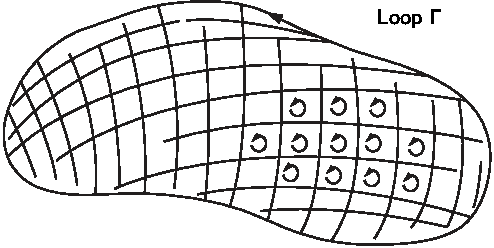
\includegraphics[width=0.7\linewidth]{fyz_fig038.pdf}
      \caption{Je zvolena nějaká plocha ohraničená uzavřenou křivkou \(\Gamma\). Plocha se rozdělí  
               na množství malých přibližně čtvercových plošek. Cirkulace po \(\Gamma\) je rovna 
               sumě cirkulací po malých uzavřených křivkách.}
      \label{fyz:fig038} 
    \end{figure}
    Nyní předpokládejme, že původní uzavřená křivka ohraničuje nějakou plochu. Ve skutečnosti 
    existuje nekonečně mnoho ploch, jež všechny mají původní křivku jako svoji hranici. Naše 
    výsledky však nebudou záviset na tom, kterou plochu zvolíme. Nejdříve rozdělíme naši původní 
    křivku na mnoho malých uzavřených křivek, jež všechny budou ležet na námi zvolené ploše, jak je 
    vidět na obr. \ref{fyz:fig038}. Zvolíme-li naše křivky dostatečně malé, můžeme, bez 
    ohledu na tvar plochy, předpokládat, že každá z nich utváří v podstatě rovinnou plošku. Kromě 
    toho můžeme křivky vybrat tak, že každá bude velmi blízká obvodu čtverce. Cirkulaci po velké 
    křivce nyní můžeme vypočítat tak, že najdeme cirkulace po obvodech všech malých čtverců a ty 
    sečteme. 

     
  %------------- CIRKULACE PO OBVODU ČTVERCE. STOKESOVA VĚTA ---------------------------------------
  \section{Cirkulace po obvodu čtverce. Stokesova věta}\hypertarget{fyz:IIchapIIIsecV}
    Jak najít cirkulaci pro každý z malých čtverečků? Závisí to na tom, jak je čtvereček 
    orientovaný v prostoru. Kdyby měl speciální orientaci, například kdyby ležel v některé ze 
    souřadnicových rovin, bylo by možné výpočet provést snadno. Protože jsme dosud o orientaci 
    souřadnicových os neudělali žádný předpoklad, můžeme si osy dobře zvolit tak, aby ten 
    čtvereček, na který je v té chvíli soustředěna naše pozornost, ležel v rovině \(xy\) (obr. 
    \ref{fyz:fig039}).
   
    Vyjádříme-li náš výsledek ve vektorové symbolice, můžeme tvrdit, že bude pro všechny konkrétní 
    orientace roviny tentýž.

    Nyní chceme najít cirkulaci pole \(\vec{C}\) po obvodu našeho malého čtverce. Křivkový 
    integrál se snadno vypočte, uděláme-li čtvereček tak malý, že podél jakékoliv jeho strany se 
    vektor \(\vec{C}\) moc nemění. (Tento předpoklad platí tím lépe, čím menší je čtvereček, takže 
    v podstatě mluvíme o infinitezimálních čtverečcích.) Vyjdeme z bodu \((x, y)\) - levého dolního 
    rohu obrázku - a budeme postupovat ve směru vyznačeném šipkami. V případě první strany, 
    označené 1, nechť je tangenciální složka \(C_x(1)\), délka dráhy nechť je \(\Delta x\). První 
    příspěvek k integrálu tedy bude \(C_x(1)\Delta x\). V případě druhé strany dostaneme 
    \(C_y(2)\Delta y\), v případě třetí \(-C_x(3)\Delta x\) a v případě čtvrté strany to bude 
    \(-C_y(3)\Delta y\). Záporná znaménka jsou nutná, neboť tangenciální složku musíme vyjadřovat 
    vzhledem ke směru postupu po obvodu. Celý křivkový integrál pak bude
    \begin{equation}\label{fyz:eq_fey_circ2}
      \oint\vec{C}\dd{\vec{s}} = C_x(1)\Delta x + C_y(2)\Delta y 
                               - C_x(3)\Delta x - C_y(3)\Delta y.
    \end{equation}      

    Všimněme si prvního a třetího členu na pravé straně. Spolu dávají
    \begin{equation}\label{fyz:eq_fey_circ3}
      [C_x(1) - C_x(3)]\Delta x.  
    \end{equation}
    Mohli byste se domnívat, že podle naší aproximace je rozdíl v hranaté závorce roven nule. Je to 
    tak, ale pouze v nulovém přiblížení. Můžeme však být přesnější a vzít v úvahu i rychlost změny 
    \(\vec{C_x}\). Když to uděláme, můžeme psát
    \begin{equation}\label{fyz:eq_fey_circ4}
      C_x(3) = C_x(1)+\pder{C_x}{y}\dd{y}.  
    \end{equation}
    Kdybychom zahrnuli následující přiblížení, vystoupily by v něm i členy obsahující \(\Delta
    y^2\). Protože však nakonec přejdeme k limitě pro \(\Delta y\rightarrow0\), je možno takové 
    členy zanedbat. Dosadíme-li (\ref{fyz:eq_fey_circ4}) do (\ref{fyz:eq_fey_circ3}), jistíme, že
    \begin{equation}\label{fyz:eq_fey_circ5}
      [C_x(1) - C_x(3)]\Delta x = -\pder{C_x}{y}\dd{x}\dd{y}.  
    \end{equation}  
    Souhlasně s naší aproximací je možno tuto derivaci počítat v bodě \((x, y)\).             

    \begin{figure}[ht!]  %\ref{fyz:fig039}
      \centering
      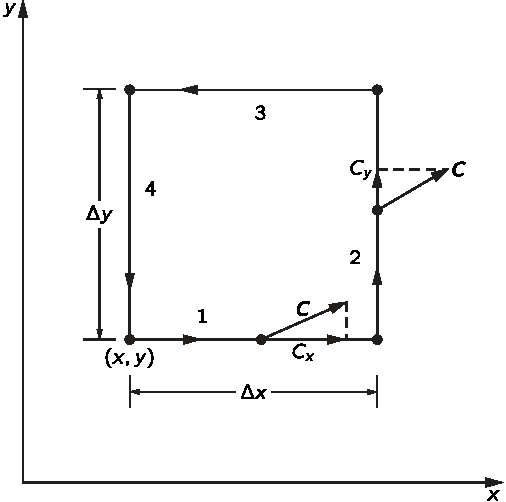
\includegraphics[width=0.7\linewidth]{fyz_fig039.pdf}
      \caption{Výpočet cirkulace \(\vec{C}\) po obvodu malého čtverečku}
      \label{fyz:fig039}
    \end{figure}
    Podobně můžeme vyjádřit zbývající dva členy ve výrazu (\ref{fyz:eq_fey_circ2}) pro cirkulaci
    \begin{equation}\label{fyz:eq_fey_circ6}
      [C_y(2) - C_y(4)]\Delta y = \pder{C_y}{x}\dd{x}\dd{y}.  
    \end{equation}    
    Cirkulace po obvodu čtverečku pak bude
    \begin{equation}\label{fyz:eq_fey_circ7}
      \left(\pder{C_y}{x}-\pder{C_x}{y}\right)\dd{x}\dd{y}.  
    \end{equation}    
    což je zajímavé, neboť rozdíl závorkách představuje právě \(z\)-ovou složku rotace. Kromě toho 
    si všimněme, že \(\Delta x\Delta y\) je plošný obsah našeho čtverečku. Takovýmto způsobem můžeme 
    naši cirkulaci (\ref{fyz:eq_fey_circ7}) psát jako
    \begin{equation}\label{fyz:eq_fey_circ8}
      (\nabla\times\vec{C})_z\dd{S}.  
    \end{equation}
    Ale \(z\)-ová složka ve skutečnosti znamená normálovou složku vzhledem k plošnému elementu. 
    Cirkulaci po obvodu diferenciálního čtverečku proto můžeme vyjádřit v invariantním vektorovém 
    tvaru:
    \begin{equation}\label{fyz:eq_fey_circ9}
      \oint\vec{C}\cdot\dd{\vec{s}} 
        = (\nabla\times\vec{C})_n\Delta S = (\nabla\times\vec{C})\cdot\vec{n}\Delta S.  
    \end{equation} 
    Náš výsledek zní: cirkulace jakéhokoliv vektoru \(\vec{C}\) po obvodu infinitezimálního 
    čtverečku je rovna normálové (vzhledem k rovině, v níž leží čtvereček) složce vektoru 
    \(\rot{C}\) vynásobené plošným obsahem čtverečku.
  
    Cirkulaci po jakékoliv uzavřené křivce \(\Gamma\) je možné nyní lehce uvést do souvislosti s 
    rotací vektorového pole. Křivku „vyplníme“ nějakou vhodnou plochou \(S\) (obr. 
    \ref{fyz:fig036}) a vypočítáme cirkulace po obvodech množiny infinitezimálních čtverečků 
    tvořících tuto plochu. Tento součet je možno zapsat jako integrál. Naším výsledkem je velmi 
    užitečná věta, nazvaná Stokesova věta (podle G. G. Stokese).
  
    \begin{flalign}
      \text{\textbf{Stokesova věta}:}                                              && 
      \oint_\Gamma\vec{C}\cdot\dd{\vec{s}} = \int_S(\nabla\times\vec{C})_n\dd{S}.  &&
    \end{flalign}
    kde \(S\) je jakákoliv plocha ohraničená křivkou \(\Gamma\). 

    \begin{figure}[ht!]  %\ref{fyz:fig036}
      \centering
      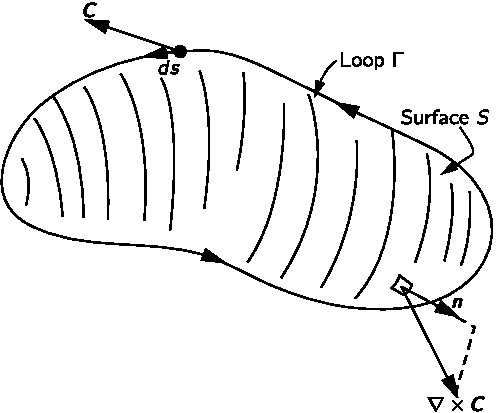
\includegraphics[width=0.7\linewidth]{fyz_fig036.pdf}
      \caption{Cirkulace \(\vec{C}\) po \(\Gamma\) je rovna plošnému integrálu normálové složky
        vektoru \(\nabla\times\vec{C}\)}
      \label{fyz:fig036}   
    \end{figure} 
    Nyní musíme něco říci o znaménkové konvenci. Na obr. \ref{fyz:fig039} směřuje osa 
    \(z\) ke čtenáři v „obyčejné“, tj. pravotočivé soustavě. Kdybychom náš křivkový integrál 
    počítali při kladné orientaci oběhu, zjistili bychom, že cirkulace je rovna \(z\)-ové složce 
    vektoru \(\nabla\times\vec{C}\). Kdybychom postupovali opačným směrem, dostali bychom opačné 
    znaménko. Jak tedy budeme obecně vědět, který směr zvolit za kladný pro normálovou složku 
    vektoru \(\nabla\times\vec{C}\)? Kladná normála musí souviset se smyslem rotace vždy tak, jak 
    je to na obr. \ref{fyz:fig039}. Obecný případ je vyznačen na obr. \ref{fyz:fig036}.

    Jedním ze způsobů, jak si tento vztah zapamatovat, je \emph{pravidlo pravé ruky}. Přiložíte-li
    \emph{pravou} ruku podél křivky \(\Gamma\) tak, že prsty ukazují kladný smysl \(\dd{\vec{s}}\), 
    palec ukazuje směr kladné normály k ploše \(S\).


  %------------- POLE S NULOVOU ROTACÍ A DIVERGENCÍ ------------------------------------------------
  \section{Pole s nulovou rotací a divergencí}\label{fyz:IIchapIIIsecVI}
    Nyní bychom se rádi zabývali některými důsledky našich nových vět. Nejdřív vezměme příklad 
    vektoru, jehož rotace je všude rovna nule. Pak je podle Stokesovy věty jeho cirkulace po každé 
    křivce také rovna nule. Z toho vyplývá, že zvolíme-li na uzavřené křivce dva body \((1)\) a 
    \((2)\) (obr. \ref{fyz:fig043}), \emph{křivkový integrál tangenciální složky z \((1)\) do 
    \((2)\) nezávisí na tom, po které ze dvou možných drah se vypočítá.} Můžeme udělat závěr, že 
    integrál z \((1)\) do \((2)\) bude záviset pouze na poloze těchto bodů, tj. je pouze nějakou 
    funkcí polohy. Stejnou logiku jsme použili v kapitole \ref{fyz:chap_fey_work}, kde jsme 
    dokázali, že když je integrál nějaké veličiny po uzavřené dráze vždy roven nule, lze jej 
    vyjádřit jako rozdíl funkce polohy dvou bodů. Tento fakt nám umožnil zavést pojem 
    \textbf{potenciálu}. Dále jsme dokázali, že \emph{vektorové pole je gradientem této 
    potenciálové funkce} (viz vztah \ref{fyz:eq008}).

    \begin{figure}[ht!]  %\ref{fyz:fig043}
      \centering
      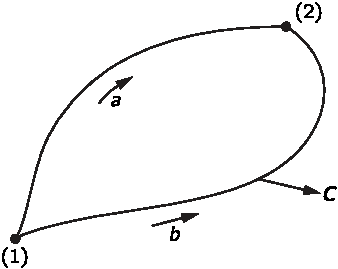
\includegraphics[width=0.6\linewidth]{fyz_fig043.pdf}
      \caption{Je-li \(\nabla\times\vec{C}\) rovno nule, cirkulace po uzavřené křivce \(\Gamma\)   
        je také rovna nule. Křivkový integrál \(\vec{C}\cdot\dd{\vec{s}}\) z (1) do (2) po 
        křivce \(a\) proto musí být stejný jako tentýž křivkový integrál po křivce \(b\).}
      \label{fyz:fig043}
    \end{figure}
    Z toho vyplývá, že každé vektorové pole s nulovou rotací je rovno gradientu nějaké skalární 
    funkce. To je užitečný poznatek: je-li \(\nabla\times\vec{C}=0\), existuje skalární pole 
    \(\Psi\) (psí), že \(\vec{C}=\nabla\Psi\). Tento zvláštní druh vektorového pole tedy můžeme, 
    chceme-li, popsat pomocí skalárního pole.
    
    Ukážeme ještě něco. Předpokládejme, že máme \emph{libovolné} skalární pole \(\varphi\) (fí). 
    Vytvoříme-li jeho gradient \(\nabla\varphi\), musí být integrál tohoto vektoru po jakékoliv 
    uzavřené křivce  roven nule. Jeho křivkový integrál z bodu \(1\) do bodu \(2\) bude 
    \(\varphi(2) - \varphi(1)\). Představují-li \(1\) a \(2\) tentýž bod, bude podle věty 1 (vztah 
    \ref{fyz:eq273}) křivkový integrál roven nule:
    \begin{equation}\label{fyz:eq359}
      \limitint_{\mathclap{\substack{\text{jakákoliv}\\\text{uzavřená}\\\text{křivka}}}}
        \nabla\varphi\dd{\vec{s}} = 0
    \end{equation}
    Na základě Stokesovy věty můžeme udělat závěř, že 
    \begin{equation}\label{fyz:eq_fey_null0} 
      \int(\nabla\times(\nabla\varphi))_n\dd{S} = 0
    \end{equation} 
    pro \emph{jakoukoliv plochu}. Je-li tento integrál roven nule pro každou plochu, musí být 
    roven nule i jeho integrand. Vždy tedy platí
    \begin{equation}
      \nabla\times(\nabla\varphi) = 0
    \end{equation}
    Tentýž výsledek jsme dokázali v článku \ref{sec:fey_diff_2deriv} pomocí vektorové algebry.      
    
       
    Nyní se podívejme na zvláštní případ, kdy malou uzavřenou křivku \(\Gamma\) vyplníme velkou 
    plochou \(S\), jako na obr. \ref{fyz:fig037}. Rádi bychom se vlastně dozvěděli, co se 
    stane, když se uzavřená křivka „scvrkne“ na bod, takže ohraničení plochy zmizí, tj. plocha se 
    stane uzavřenou. Je-li vektor \(\vec{C}\) všude konečný, musí se při „scvrkávání“ křivky 
    \(\Gamma\) křivkový integrál po \(\Gamma\) blížit nule (integrál je přibližně přímo úměrný 
    délce \(\Gamma\) která se blíží nule). Podle Stokesovy věty se musí plošný integrál veličiny 
    \((\nabla\times\vec{C})_n\) také blížit nule. Když plochu uzavíráme, jako bychom přidávali 
    příspěvky, které postupně vyruší to, co bylo předtím. Dospěli jsme k nové větě
    \begin{equation}\label{fyz:eq_fey_null1} 
      \limitoint_{\mathclap{\substack{\text{jakákoliv}\\\text{uzavřená}\\\text{křivka}}}}
       (\nabla\times\vec{C})_n \dd{s} = 0
    \end{equation}

    \begin{figure}[ht!]  %\ref{fyz:fig037}
      \centering
      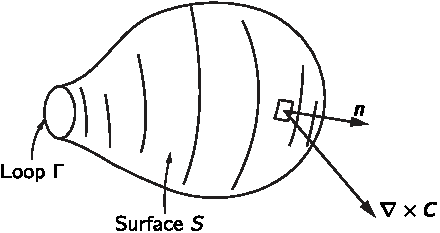
\includegraphics[width=0.7\linewidth]{fyz_fig037.pdf}
      \caption{Přechodem k limitnímu případu uzavřené plochy zjistíme, že plošný integrál veličiny
               \((\nabla\times\vec{C})_n\) musí konvergovat k nulové hodnotě.
               \cite[s.~60]{Feynman02}}
      \label{fyz:fig037}
    \end{figure}
    Nyní je to zajímavé, neboť jednu větu o plošném integrálu uzavřenou plochou už máme. Takový 
    plošný integrál je podle Gaussovy věty (vztah \ref{fyz:eq_gauss_veta}) roven objemovému 
    integrálu divergence vektorového pole. Z Gaussovy věty použité na vektor 
    \(\nabla\times\vec{C}\) vyplývá
    \begin{equation}\label{fyz:eq_fey_null2} 
      \limitint_{\mathclap{\substack{\text{uzavřená}\\\text{plocha}}}}
       (\nabla\times\vec{C})_n \dd{\vec{S}}
      =
      \limitint_{\mathclap{\substack{\text{objem uvnitř}\\\text{plochy}}}}
        \nabla\cdot(\nabla\times\vec{C})\dd{V}.
    \end{equation}
    Z toho usuzujeme, že druhý integrál musí být též roven nule:
    \begin{equation}\label{fyz:eq_fey_null3} 
     \limitint_{\mathclap{\substack{\text{jakýkoliv}\\\text{objem}}}}
      \nabla\cdot(\nabla\times\vec{C})\dd{V} = 0
    \end{equation}
            
    To také platí pro každé vektorové pole \(\vec{C}\). Protože však rovnost 
    (\ref{fyz:eq_fey_null3}) je správná pro \emph{každý objem}, musí platit, že v každém bodě 
    prostoru je integrand roven nule. Dostáváme, že vždy
    \begin{equation}\label{fyz:eq_fey_null4}
     \nabla\cdot(\nabla\times\vec{C})=0.
    \end{equation}
    To je však stejný výsledek, jaký jsme dostali v článku \ref{sec:fey_diff_2deriv} z vektorové 
    algebry. Nyní začínáme chápat, jak jedno souvisí s druhým.      
 
  %---------------------- Shrnutí ------------------------------------------------------------------
  \section{Shrnutí}
    Shrňme, co jsme se dozvěděli o vektorovém počtu. Skutečně významné výsledky kapitol
    \ref{fyz:IIchapII} a \ref{fyz:IIchapIII} jsou tyto:
    \begin{enumerate}[noitemsep]
      \item Operátory \(\pder{ }{x}\), \(\pder{ }{y}\) a  \(\pder{ }{z}\) možno považovat za tři
            složky vektorového operátoru:
            \begin{equation}
               \nabla = \left(\pder{ }{x}, \pder{ }{y}, \pder{ }{z}\right)
            \end{equation}
            Zachází-li se s tímto operátorem jako s vektorem, vzorce, které pro něj vyplývají z
            vektorové algebry, jsou správné.
      \item Rozdíl hodnot skalárního pole ve dvou bodech je roven křivkovému integrálu tangenciální
            složky gradientu tohoto skaláru po jakékoliv křivce spojující oba body:
            \begin{equation}
              \Psi(2)-\Psi(1) = 
                \limitint_{\mathclap{\substack{(1)\\\text{jakákoli}\\\text{křivka}}}}^{(2)}
                \nabla\Psi\cdot\dd{\vec{s}}
            \end{equation}
      \item Plošný integrál normálové složky libovolného vektoru po uzavřené ploše je roven 
            integrálu divergence tohoto vektoru přes vnitřní objem ohraničený plochou:
            \begin{equation}
              \limitint_{\mathclap{\substack{\text{uzavřená}\\\text{plocha}}}}          
                         \vec{C}\cdot\vec{n}\dd{S} 
            = \limitint_{\mathclap{\substack{\text{objem}\\\text{uvnitř}\\\text{plochy}}}} 
                        (\nabla\cdot\vec{C})\dd{V}, 
            \end{equation}
      \item Křivkový integrál tangenciální složky libovolného vektoru po uzavřené křivce je roven
            plošnému integrálu normálové složky rotace tohoto vektoru po jakékoliv ploše, která je
            touto křivkou ohraničena:
            \begin{equation}
              \limitint_{\mathclap{\substack{\text{hranice}}}}  
                \vec{C}\cdot\dd{\vec{s}} =
              \limitint_{\mathclap{\substack{\text{plocha}}}}
                (\nabla\times\vec{C})\cdot\vec{n}\dd{S}.
            \end{equation}            
    \end{enumerate}
      
  %------------- Vizualizace vektorového pole s využitím šumové textury ----------------------------
%  \tikzexternaldisable
  \section{Vizualizace vektorového pole s využitím šumové textury}
    Záměrem této „názorné exkurze“ do teorie pole je poskytnout náhled s využitím animací. 
    Zopakujme že, vektor je veličina, která určuje nejen velikost, ale i směr v prostoru. Vektory 
    tedy používáme k popisu fyzikálních veličin, jako je např. rychlost, hybnost, zrychlení nebo 
    síla působící na objekt. Nicméně, pokud se pokoušíme popsat systém, který se skládá z velkého 
    počtu objektů (např. pohybující se voda, sníh, déšť,…), musíme přiřadit vektor každému 
    samostatnému objektu. Například v každém okamžiku můžeme jakékoliv sněhové vločce přiřadit 
    vektor rychlosti, který charakterizuje její pohyb. Padající sníh je příkladem diskrétního, tj. 
    nespojitého prostředí.    
    
    Stejné je to u analýzy pohybu tekutiny. I v tomto případě musíme vektor rychlosti přiřadit v 
    každém okamžiku každé částečce tekutiny. Takto budou vektory popisovat směr a velikost 
    rychlosti v každém čase a v každém bodě prostoru. Soubor všech vektorů rychlosti nazveme 
    \emph{vektorovým polem} rychlostí. Nyní je jasný podstatný rozdíl mezi vektorovým a skalárním 
    polem tj., že vektorové obsahuje informaci jak o velikosti, tak i o směru veličiny v každém 
    časovém okamžiku pro každý bod v prostoru, zatímco skalární pouze udává velikost dané veličiny 
    v každém čase a v každém bodě prostoru. Příkladem spojitého prostředí je např. proudění vzduchu.
    
    Obecné vektorové pole \(\vec{F}(x, y, z)\) můžeme napsat ve tvaru:
    \begin{equation}
     \vec{F}(x,y,z) = F_x(x,y,z)\vec{i} + F_y(x,y,z)\vec{j} + F_z(x,y,z)\vec{k},
    \end{equation} 
    kde jednotlivé komponenty jsou \emph{skalární pole}. Pro ilustraci vlastností vektorových polí 
    použijeme tekutinové pole, protože vizualizace takovýchto typů vektorových polí jsou 
    nejjednodušší.  
    
    Zobrazení vektorových polí je provedeno pomocí šumové textury, která je lokálně korelována se 
    směrem vektorového pole. Obdobné zobrazení lze přirozeným způsobem realizovat i experimentálně. 
    Rozházíme-li semínka trávy v silném elektrickém poli, začnou se orientovat delší osou 
    rovnoběžně se směrem silokřivek pole. Poskytnou nám tím hustý soubor vzorků zobrazujících směry 
    a tedy i tvar pole. Platí tedy, že lokální směry polí jsou v souhlase se směry šumové textury 
    diagramu. Šumová textura umí poskytnout mnoho informací o prostorové struktuře pole.

    \begin{figure}[ht!]
      \centering
      \AddVideo{160}{130}{vf_div}
      \caption{Proudové pole má zřídlo v počátku souřadnic a proudnice od něho směřují radiálně} 
      \label{FYZ:fig_fey_anim1}
    \end{figure}

    \begin{figure}[ht!]
      \centering 
      \AddVideo{160}{130}{vf_curl} 
      \caption{Proudové pole je vytvářeno pouze vírem; je bez zřídla, tekutina se pohybuje po 
               kružnicích a nedochází ani ke vzniku, ani k zániku částic tekutiny} 
      \label{FYZ:fig_fey_anim2}
    \end{figure}
    
    První animace \ref{FYZ:fig_fey_anim1} znázorňuje \emph{divergující tok} tekutiny, šumovou 
    texturou, jejíž směr je v korelaci se směrem tohoto toku. Animace na obr. 
    \ref{FYZ:fig_fey_anim2} zobrazuje jinou třídu chování toku tekutiny  - \emph{cirkulaci, 
    víření}. Kapalina se pohybuje jednoduše v kruzích, nic zde nevzniká ani nezaniká (nemá zdroj 
    ani propad).   

    Na animaci \ref{FYZ:fig_fey_anim3} je zřídlo v blízkosti menší výpusti (propadu), zatímco 
    animace \ref{FYZ:fig_fey_anim4} znázorňuje dvě zřídla nestejné síly. Tekutinové pole může mít 
    více než jeden střed víření. 

    \begin{figure}[ht!]
      \centering
      \AddVideo{160}{130}{vf_divdiv1} 
      \caption{Proudové pole je složeno ze zřídla a z propadu (tzv. proudový dipól); v okolí 
               zřídla a propadu směřují proudnice vždy od zřídla směrem k propadu}
      \label{FYZ:fig_fey_anim3}
    \end{figure}

    Na animaci \ref{FYZ:fig_fey_anim5} je ukázán tok pole se dvěma víry, cirkulacemi. Toky víří v 
    opačných směrech a jeden je silnější než druhý. Na animaci \ref{FYZ:fig_fey_anim6} máme stejnou 
    situaci, ale směry obou vírů jsou stejné.    
    
    Na animaci \ref{FYZ:fig_fey_anim7} je ukázán konstantní tok klesající dolů, který se vzájemně 
    ovlivňuje se zřídlem. Zdroj je částečně schopen téci vzhůru proti proudu padající tekutiny, ale 
    nakonec je také stržen a otočen směrem dolů.
    
    Podobně na animaci \ref{FYZ:fig_fey_anim8} je znázorněn homogenní tok směřující dolů, 
    interagující s tokem cirkulujícím proti směru hodinových ručiček. Otáčivý tok je schopen téci 
    kousek proti proudu, ale nakonec je stržen silnějším tokem směrem dolů.

    \begin{figure}[ht!]
      \centering
      \AddVideo{160}{130}{vf_divdiv2} 
      \caption{Proudového pole je v reálném čase deformováno ve směru rychlostního pole a je 
               složeno ze dvou různě silných zřídel v různých místech; v blízkém okolí obou zřídel 
               se proudnice pohybují směrem od zřídel}
      \label{FYZ:fig_fey_anim4}
    \end{figure} 

    \begin{figure}[ht!]
      \centering  
      \AddVideo{160}{130}{vf_curlcurl2}  
      \caption{Proudového pole je v reálném čase deformována ve směru rychlostního pole a je 
               složeno ze dvou různě silných vírů v různých místech; směr rotace jednoho víru je ve 
               směru hodinových ručiček a druhého proti směru hodinových ručiček}
      \label{FYZ:fig_fey_anim5}
    \end{figure} 

    \begin{figure}[ht!]
      \centering
      \AddVideo{160}{130}{vf_curlcurl1} 
      \caption{Proudového pole je v reálném čase deformována ve směru rychlostního pole a je  
               složeno ze dvou různě silných vírů v různých místech; směr rotace obou vírů je v 
               tomto případě shodný}
      \label{FYZ:fig_fey_anim6}
    \end{figure} 
    
    Konečně na animaci \ref{FYZ:fig_fey_anim9} jsou ukázány oba toky pole, jak vír, tak i zdroj 
    (jak rotace, tak také divergence vektorového pole jsou nenulové). Jakékoli vektorové pole lze 
    zapsat jako součet nevírových částí (nulová rotace) a nedivergujících (nezřídlových, 
    nezdrojových) částí (žádná zřídla ani propady částic). V našem studiu elektromagnetizmu 
    uvidíme, že\emph{ statické elektrické pole je nevírové} (tj. vypadá jako na animacích 
    \ref{FYZ:fig_fey_anim1}, \ref{FYZ:fig_fey_anim3}, \ref{FYZ:fig_fey_anim4} a 
    \ref{FYZ:fig_fey_anim7}) a \emph{statické magnetické pole je nedivergující, nezdrojové} (tj. 
    podobá se animacím \ref{FYZ:fig_fey_anim2}, \ref{FYZ:fig_fey_anim5}, \ref{FYZ:fig_fey_anim6} a 
    \ref{FYZ:fig_fey_anim8}). Jenom v případech časově proměnného elektrického pole můžeme 
    pozorovat, že má elektrické pole obě vlastnosti, tj. je jak zdrojové, tak i vírové, takže 
    vypadá jako na animaci \ref{FYZ:fig_fey_anim9}. Narozdíl od pole elektrického je pole 
    magnetické vždy nezdrojové (nedivergentní), a to i v časově proměnných situacích. To znamená, 
    že magnetické pole se vždy podobá modelům z animacím \ref{FYZ:fig_fey_anim2}, 
    \ref{FYZ:fig_fey_anim5}, \ref{FYZ:fig_fey_anim6} a \ref{FYZ:fig_fey_anim8}.              
    
    \begin{figure}[ht!]
      \centering
      \AddVideo{160}{130}{vf_divconstant}   
      \caption{Proudového pole je v reálném čase deformována ve směru  
               rychlostního pole a je vytvářeno zřídlem umístěným v 
               homogenním konstantním toku, který míří shora dolů 
               (tzv. Rankinovo polotěleso, Rankinův ovál)}
      \label{FYZ:fig_fey_anim7}
    \end{figure}

    \begin{figure}[ht!]
      \centering
      \AddVideo{160}{130}{vf_curlconstant}    
      \caption{Proudového pole je v reálném čase deformována ve směru   
               rychlostního pole a je složeno z víru a homogenního toku 
               směřujícího shora dolů}
      \label{FYZ:fig_fey_anim8}
    \end{figure}

    \begin{figure}[ht!]
      \centering 
      \AddVideo{160}{130}{vf_divcurl}
      \caption{Proudového pole je v reálném čase deformována ve směru    
               rychlostního pole a je vytvářeno kombinací víru a zřídla}
      \label{FYZ:fig_fey_anim9}
    \end{figure}
%    \tikzexternalenable

%} %tikzset
%~~~~~~~~~~~~~~~~~~~~~~~~~~~~~~~~~~~~~~~~~~~~~~~~~~~~~~~~~~~~~~~~~~~~~~~~~~~~~~~~~~~~~~~~~~~~~~~~~~
